\documentclass[12pt,a4paper,fleqn]{article}
\title{Progress Report}
\author{Syed Ahmad Raza}
\date{2018.03.21}
\usepackage{mathtools}
\usepackage{graphicx}
\usepackage{color}          % for color eps output
% \usepackage{afterpage}
\usepackage{float}          % to force a figure placement with [H] command
\usepackage{enumitem}
\usepackage{newtxtext}
\usepackage{newtxmath}
\usepackage{nicefrac}
%\usepackage{layouts}       % for: \printinunitsof{in}\prntlen{\textwidth}

\begin{document}
\maketitle
%\tableofcontents
\pagebreak

\section{Numerical solution of cavity flow problem using\\
    Finite Volume Method}

\subsection{Graphical results for cavity flow problem}

The cavity flow problem was solved using Finite Volume Method by coding a solution in C++. The results are presented below.

\begin{figure}[H]
    \centering
%    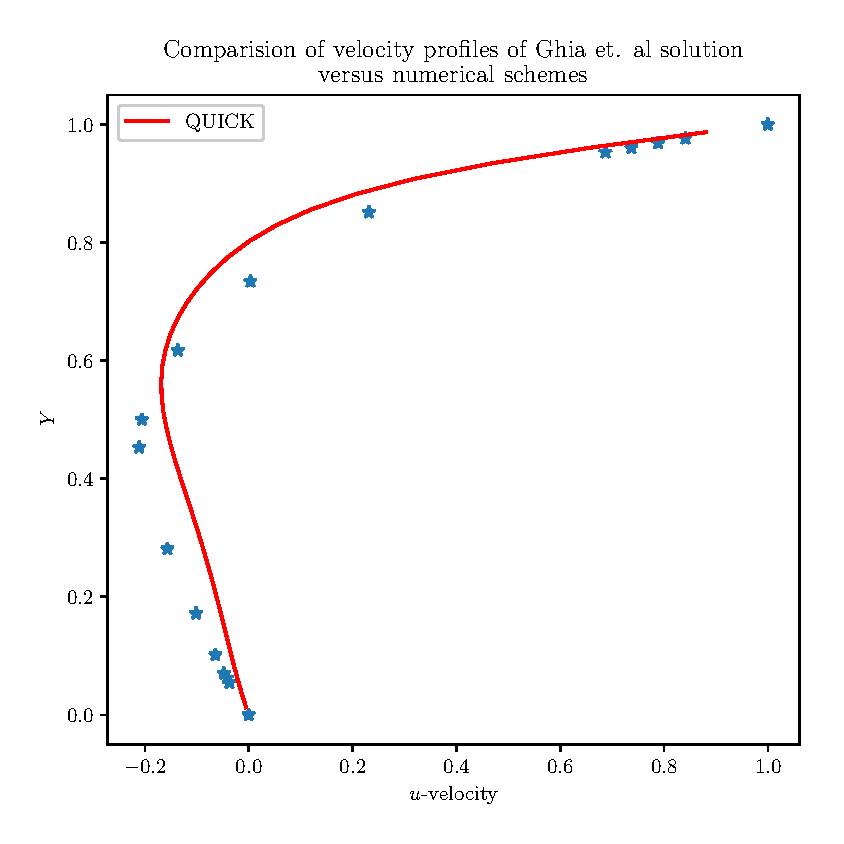
\includegraphics[width=\textwidth]{n,xy=40_qk_cavityFlowY.eps}
    \label{fig:n,xy=40_qk_cavityFlowY.eps}
\end{figure}

\begin{figure}[H]
    \centering
%    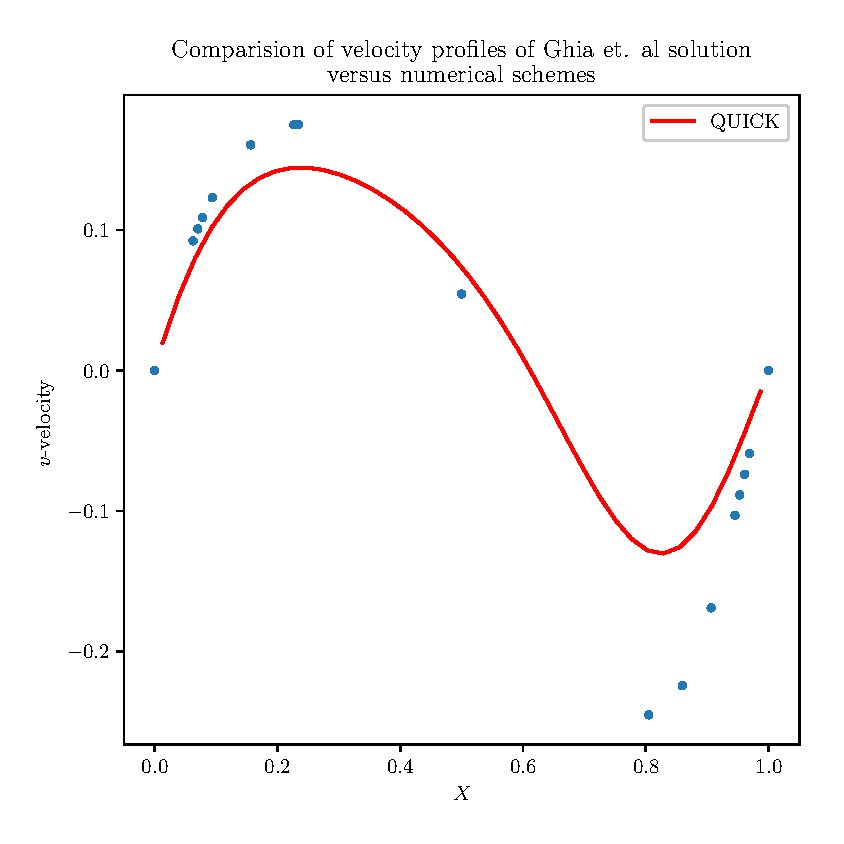
\includegraphics[width=\textwidth]{n,xy=40_qk_cavityFlowX.eps}
    \label{fig:n,xy=40_qk_cavityFlowX.eps}
\end{figure}

\begin{figure}[H]
    \centering
%    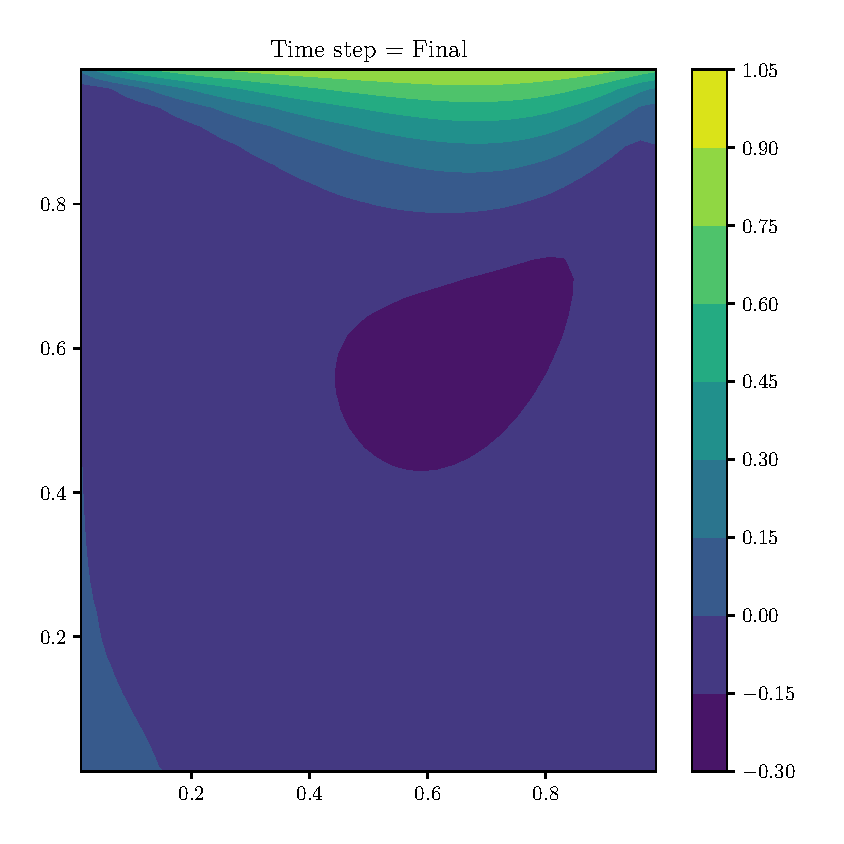
\includegraphics[width=\textwidth]{n,xy=40_qk_uContours.eps}
    \label{fig:n,xy=40_qk_uContours.eps}
\end{figure}

\begin{figure}[H]
    \centering
%    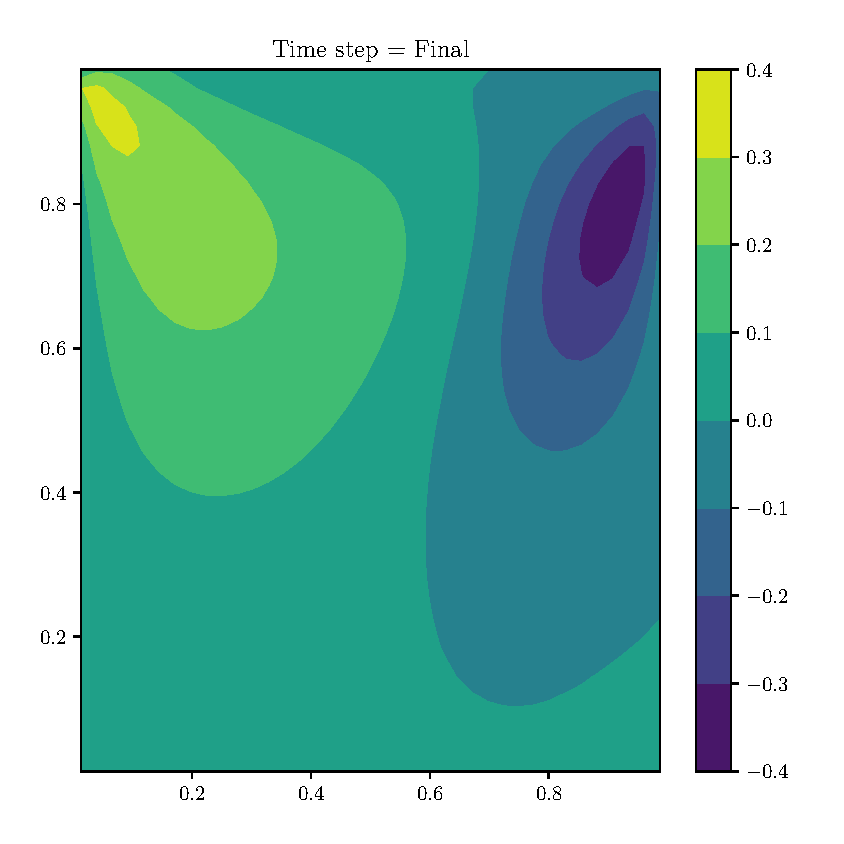
\includegraphics[width=\textwidth]{n,xy=40_qk_vContours.eps}
    \label{fig:n,xy=40_qk_vContours.eps}
\end{figure}

\begin{figure}[H]
    \centering
%    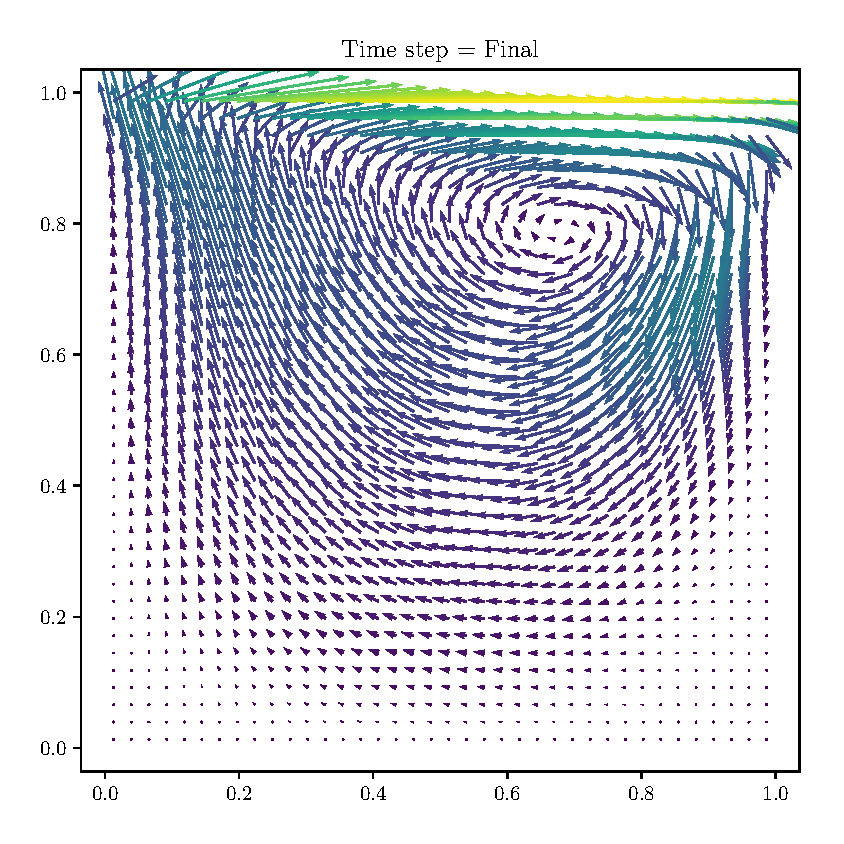
\includegraphics[width=\textwidth]{n,xy=40_qk_velVectors.eps}
    \label{fig:n,xy=40_qk_velVectors.eps}
\end{figure}

\subsection{Discretization of the convective and diffusive terms for 2D nonuniform grid}

\begin{figure}[H]
    \centering
    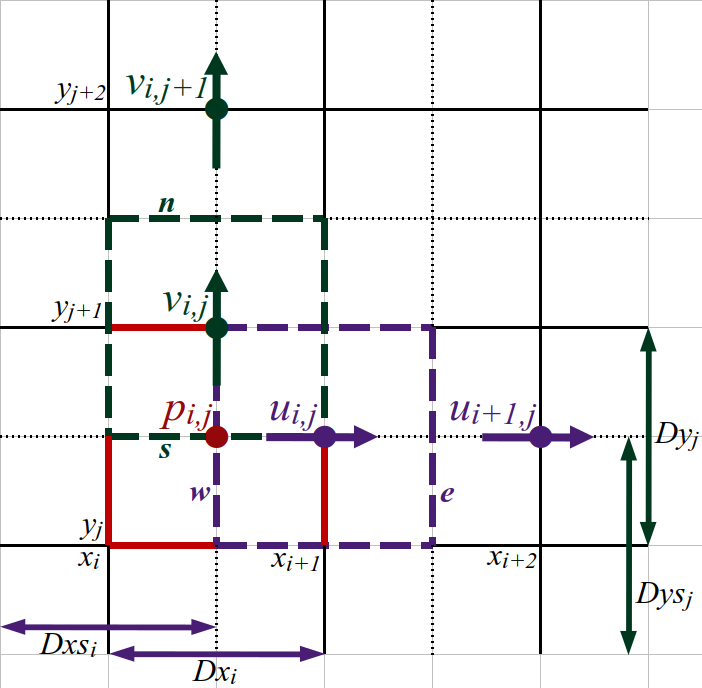
\includegraphics[width=0.5\textwidth]{staggered_grid.png}
    \caption{Visual representation of the staggered grid used for discretization in Finite Volume Method}
    \label{fig:staggered-grid}
\end{figure}

Linear interpolation is used for the velocities \(u_n, u_s, v_e,\) and \(v_w\). Let us analyze one of the velocities \(u_n\).

\begin{equation*}
\frac{u_n - u_{i,j}}{y_{j+1} - y_{j+\nicefrac{1}{2}}}
= \frac{u_{i,j+1} - u_{i,j}}{y_{j+\nicefrac{3}{2}} - y_{j+\nicefrac{1}{2}}}
\end{equation*}
\begin{equation*}
\frac{u_n - u_{i,j}}{\nicefrac{Dy_j}{2}}
= \frac{u_{i,j+1} - u_{i,j}}
{\left(\nicefrac{Dy_{j+1}}{2}\right) + \left(\nicefrac{Dy_j}{2}\right)}
\end{equation*}
\begin{equation*}
\frac{u_n - u_{i,j}}{\nicefrac{Dy_j}{2}}
= \frac{u_{i,j+1} - u_{i,j}}
{\nicefrac{\left(Dy_{j+1} +Dy_j\right)}{2}}
\end{equation*}

Therefore, the terms reduce to the following:
\begin{equation*}
\begin{aligned}
u_n &= u_{i,j} + \left(\frac{u_{i,j+1} - u_{i,j}}{Dys_{j+1}}\right)
\left(\frac{Dy_j}{2}\right)\\
u_s &= u_{i,j-1} + \left(\frac{u_{i,j} - u_{i,j-1}}{Dys_j}\right)
\left(\frac{Dy_{j-1}}{2}\right)
\end{aligned}
\qquad
\begin{aligned}
v_e &= v_{i,j} + \left(\frac{v_{i+1,j} - v_{i,j}}{Dxs_{i+1}}\right)
\left(\frac{Dx_i}{2}\right)\\
v_w &= v_{i-1,j} + \left(\frac{v_{i,j} - v_{i-1,j}}{Dxs_i}\right)
\left(\frac{Dx_{i-1}}{2}\right)
\end{aligned}
\end{equation*}

\subsubsection{Upwind scheme for velocities in the convective terms}
For rest of the velocities in convective terms, the upwind scheme may be used. For positive velocities,
\begin{equation*}
\begin{aligned}
u_e &= u_{i,j}\\
v_n &= v_{i,j}
\end{aligned}
\qquad\qquad
\begin{aligned}
u_w &= u_{i-1,j}\\
v_s &= v_{i,j-1}
\end{aligned}
\qquad\qquad
\begin{aligned}
u_{e,v} &= u_{i,j}\\
v_{n,u} &= v_{i,j}
\end{aligned}
\qquad\qquad
\begin{aligned}
u_{w,v} &= u_{i-1,j}\\ 
v_{s,u} &= v_{i,j-1}
\end{aligned}
\end{equation*}
For negative velocities,
\begin{equation*}
\begin{aligned}
u_e &= u_{i+1,j}\\
v_n &= v_{i,j+1}
\end{aligned}
\qquad\qquad
\begin{aligned}
u_w &= u_{i,j}\\
v_s &= v_{i,j}
\end{aligned}
\qquad\qquad
\begin{aligned}
u_{e,v} &= u_{i,j+1}\\
v_{n,u} &= v_{i+1,j}
\end{aligned}
\qquad\qquad
\begin{aligned}
u_{w,v} &= u_{i-1,j+1}\\ 
v_{s,u} &= v_{i+1,j-1}
\end{aligned}
\end{equation*}

For the first time step, Euler scheme is used and for subsequent time steps, Adams-Bashforth scheme is utilized.

\subsubsection{QUICK scheme for velocities in the convective terms}
QUICK scheme is also incorporated in the code, with an option to switch between upwind (first order) or QUICK scheme (second order). For positive velocities,
\begin{equation*}
u_e = \frac{u_{i} + u_{i+1}}{2} - \frac{Dx_{i+1}^2}{8Dxs_{i+1}}
\left(\frac{u_{i+1} - u_{i}}{Dx_{i+1}} - \frac{u_{i} - u_{i-1}}{Dx_{i}}\right)
\end{equation*}
\begin{equation*}
u_w = \frac{u_{i-1} + u_{i}}{2} - \frac{Dx_{i}^2}{8Dxs_{i}}
\left(\frac{u_{i} - u_{i-1}}{Dx_{i}} - \frac{u_{i-1} - u_{i-2}}{Dx_{i-1}}\right)
\end{equation*}
\begin{equation*}
v_n = \frac{v_{j} + v_{j+1}}{2} - \frac{Dy_{j+1}^2}{8Dys_{j+1}}
\left(\frac{v_{j+1} - v_{j}}{Dy_{j+1}} - \frac{v_{j} - v_{j-1}}{Dy_{j}}\right)
\end{equation*}
\begin{equation*}
v_s = \frac{v_{j-1} + v_{j}}{2} - \frac{Dy_{j}^2}{8Dys_{j}}
\left(\frac{v_{j} - v_{j-1}}{Dy_{j}} - \frac{v_{j-1} - v_{j-2}}{Dy_{j-1}}\right)
\end{equation*}

For negative velocities,
\begin{equation*}
u_e = \frac{u_{i} + u_{i+1}}{2} - \frac{Dx_{i+1}^2}{8Dxs_{i+2}}
\left(\frac{u_{i+2} - u_{i+1}}{Dx_{i+2}} - \frac{u_{i+1} - u_{i}}{Dx_{i+1}}
\right)
\end{equation*}
\begin{equation*}
u_w = \frac{u_{i-1} + u_{i}}{2} - \frac{Dx_{i}^2}{8Dxs_{i+1}}
\left(\frac{u_{i+1} - u_{i}}{Dx_{i+1}} - \frac{u_{i} - u_{i-1}}{Dx_{i}}\right)
\end{equation*}
\begin{equation*}
v_e = \frac{v_{j} + v_{j+1}}{2} - \frac{Dy_{j+1}^2}{8Dys_{j+2}}
\left(\frac{v_{j+2} - v_{j+1}}{Dy_{j+2}} - \frac{v_{j+1} - v_{j}}{Dy_{j+1}}
\right)
\end{equation*}
\begin{equation*}
v_w = \frac{v_{j-1} + v_{j}}{2} - \frac{Dy_{j}^2}{8Dys_{j+1}}
\left(\frac{v_{j+1} - v_{j}}{Dy_{j+1}} - \frac{v_{j} - v_{j-1}}{Dy_{j}}\right)
\end{equation*}

\newpage

\subsection{Future work}
\begin{itemize}
\item Generate figures for 3D grid
\item Apply grid average and nodal value in QUICK scheme
\item Use Smagorinsky-Lilly turbulent model for 2D case
\end{itemize}

\end{document}
